\documentclass[letterpaper,11pt]{article}
% Compilar con PDFLaTeX

% Paquetes esenciales
\usepackage{amsmath,amssymb,amsfonts}
\usepackage[spanish]{babel}
\usepackage{graphicx}
\usepackage[utf8]{inputenc}
\usepackage{enumitem}
\usepackage{multicol}
\usepackage{tasks}
\usepackage[thinlines]{easytable}
% Paquetes adicionales
\usepackage{booktabs}
\usepackage{mdwlist}
\usepackage{scalerel} %para escalar tamaños
\usepackage[margin=2.0cm]{geometry}
\usepackage[mathscr]{euscript}
\usepackage{siunitx}
\sisetup{output-decimal-marker = {,}}
% PGF/TikZ setup
\usepackage{pgfplots}
\pgfplotsset{compat=newest}
% Titling
\usepackage{titling}
\setlength{\droptitle}{-1.5cm}
% Algunas definiciones



\begin{document}
\pagestyle{empty} %quita numeracion de paginas

Una corriente de 100[mA] vaja por el alambre de la figura desde el punto + hasta el punto - . Calcule el campo magnético en el origen del sistema coordenado generado por dicha corriente.

Considere que: Radio Menor = 10.0[cm] y Radio Mayor = 20.0[cm].

\begin{minipage}{0.55\columnwidth}
 \centering
 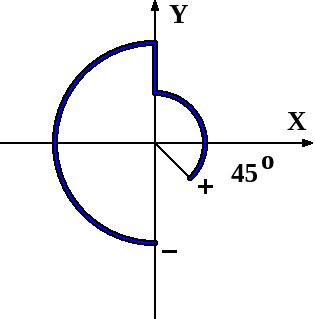
\includegraphics[width=.7\columnwidth]{Alam.png}
\end{minipage}

Resolvemos por Biot-savat, todo en cartesiano.

\begin{equation*}
\vec{B}=\int \frac{\mu_0}{4\pi} \frac{I(\vec{dl}\times\hat{r'})}{r'^2}
\end{equation*}

Primer tramo\\

Primero definimos donde están nuestros difereciales de corriente:\\
$\vec{r_I}=R\cos(\theta)\hat{x}+R\sin(\theta)\hat{y}$ con $-\pi/4<\theta<\pi/2$\\
Luego calculamos nuestro vector $\vec{r'}$\\
$\vec{r'}=0-\vec{r_I}=-R\cos(\theta)\hat{x}-R\sin(\theta)\hat{y}$\\
De aquí la magnitud del vector es:\\
$r'=\sqrt{(R\cos(\theta))^2+(R\sin(\theta))^2)}=R$\\
Luego el vector unitario es:\\
$\hat{r'}=\frac{\vec{r'}}{r'}=-\cos(\theta)\hat{x}-\sin(\theta)\hat{y}$\\
Finalmente el diferencial $\vec{dl}$ se obtiene diferenciando $\vec{r_I}$\\
$\vec{dl}=d\vec{r_I}=-R\sin(\theta)d\theta\hat{x}+R\cos(\theta)d\theta\hat{y}$\\
Ahora reemplazamos en la exuación de Biot Savat\\
\begin{equation*}
\vec{B}=\int_{-\pi/4}^{\pi/2} \frac{\mu_0}{4\pi} \frac{I((-R\sin(\theta)d\theta\hat{x}+R\cos(\theta)d\theta\hat{y})\times(-\cos(\theta)\hat{x}-\sin(\theta)\hat{y}))}{R^2}
\end{equation*}
\begin{equation*}
\vec{B}=\int_{-\pi/4}^{\pi/2} \frac{\mu_0}{4\pi} \frac{IR(\sin(\theta)^2+\cos(\theta)^2)}{R^2}d\theta
\end{equation*}
$\vec{B}=\frac{\mu_0 I}{4\pi R} \frac{3\pi}{4}\hat{z}=\frac{3}{16} \frac{\mu_0 I}{R}\hat{z}=2.36\times 10^{-7} T \hat{z}$ \textcolor{red}{(7 Puntos)}\\

Segundo tramo\\

Primero definimos donde están nuestros difereciales de corriente:\\
$\vec{r_I}=y\hat{y}$ con $0.1m<y<0.2m$\\
Luego calculamos nuestro vector $\vec{r'}$\\
$\vec{r'}=0-\vec{r_I}=-y\hat{y}$\\
De aquí la magnitud del vector es:\\
$r'=\sqrt{(y)^2}=y$\\
Luego el vector unitario es:\\
$\hat{r'}=\frac{\vec{r'}}{r'}=-\hat{y}$\\
Finalmente el diferencial $\vec{dl}$ se obtiene diferenciando $\vec{r_I}$\\
$\vec{dl}=d\vec{r_I}=-dy\hat{y}$\\
Ahora reemplazamos en la exuación de Biot Savat\\
\begin{equation*}
\vec{B}=\int_{0.1m}^{0.2m} \frac{\mu_0}{4\pi} \frac{I((-dy\hat{y})\times(-y\hat{y}))}{y^2}=0  \textcolor{red}{(3 Puntos)}
\end{equation*}

Tercer tramo\\

Primero definimos donde están nuestros difereciales de corriente:\\
$\vec{r_I}=R\cos(\theta)\hat{x}+R\sin(\theta)\hat{y}$ con $\pi/2<\theta<3\pi/2$\\
Luego calculamos nuestro vector $\vec{r'}$\\
$\vec{r'}=0-\vec{r_I}=-R\cos(\theta)\hat{x}-R\sin(\theta)\hat{y}$\\
De aquí la magnitud del vector es:\\
$r'=\sqrt{(R\cos(\theta))^2+(R\sin(\theta))^2)}=R$\\
Luego el vector unitario es:\\
$\hat{r'}=\frac{\vec{r'}}{r'}=-\cos(\theta)\hat{x}-\sin(\theta)\hat{y}$\\
Finalmente el diferencial $\vec{dl}$ se obtiene diferenciando $\vec{r_I}$\\
$\vec{dl}=d\vec{r_I}=-R\sin(\theta)d\theta\hat{x}+R\cos(\theta)d\theta\hat{y}$\\
Ahora reemplazamos en la exuación de Biot Savat\\
\begin{equation*}
\vec{B}=\int_{\pi/2}^{3\pi/2} \frac{\mu_0}{4\pi} \frac{I((-R\sin(\theta)d\theta\hat{x}+R\cos(\theta)d\theta\hat{y})\times(-\cos(\theta)\hat{x}-\sin(\theta)\hat{y}))}{R^2}
\end{equation*}
\begin{equation*}
\vec{B}=\int_{\pi/2}^{3\pi/2} \frac{\mu_0}{4\pi} \frac{IR(\sin(\theta)^2+\cos(\theta)^2)}{R^2}d\theta
\end{equation*}
$\vec{B}=\frac{\mu_0 I}{4\pi R} \pi\hat{z}=\frac{\mu_0 I}{4R}\hat{z}=1.57\times 10^{-7} T \hat{z} \textcolor{red}{(7 Puntos)}$\\

Campo magnético total\\

$\vec{B}=2.36\times 10^{-7} T \hat{z} + 1.57\times 10^{-7} T \hat{z}=3.93\times 10^{-7} T \hat{z} \textcolor{red}{(3 Puntos)}$

\end{document}
